\documentclass[UTF8]{ctexart}
\usepackage{amsmath}
\usepackage{amssymb}
\usepackage{booktabs}
\usepackage{background}
\usepackage{caption,subcaption}
\usepackage{enumitem}
\usepackage{fancyhdr}
\usepackage{float}
\usepackage{fontspec}
%\usepackage{fourier}
\usepackage{geometry}
\usepackage{listings}
\usepackage{pifont}
\usepackage{tasks}
\usepackage{tikz}
\usetikzlibrary{arrows.meta, positioning, shapes.geometric, calc}
\usepackage[dvipsnames]{xcolor}

\geometry{a5paper, top=0.1cm, left=1cm, right=1cm, bottom=1cm, footskip=0.1cm}
\setCJKmainfont[BoldFont={汉仪文黑-85W},ItalicFont={方正苏新诗柳楷简体}]{汉仪文黑-55W}
\setfontfamily\Issue{Century Schoolbook}
\setfontfamily\Genshin{Genshin Teyvat Lingua Franca}
\newCJKfontfamily\TitleFont{思源宋体 CN Heavy}
\newfontfamily\timesnewroman{Times New Roman}

\pagestyle{fancy}
\fancyhf{}
\cfoot{\sffamily\footnotesize{-\ \thepage\ -}}
\CTEXsetup[format={\bfseries\large}]{paragraph}
%\CTEXsetup[format = {\centering\bfseries\large}, beforeskip = 3pt, afterskip = 3pt]{section}

\colorlet{darkcyan}{cyan!50!black}
\newcommand\Black[1]{\textcolor[gray]{0.3}{#1}}
\newcommand\Brown[1]{\textcolor[HTML]{998A4E}{#1}}
\newcommand\Emph[1]{\colorbox{green!10}{\textcolor{green!30!black}{#1}}}
\newcommand\Notes[1]{\textcolor{yellow!50!black}{\small #1}}
\newcommand\Example[1]{\textcolor{cyan!70!black}{\small #1}}
\settasks{ label=(\Alph*), item-format=\color{darkcyan}, label-format=\color{darkcyan}, label-offset=0.7em}


\lstset{
    basicstyle=\small\ttfamily, %注意行末有逗号!
    keywordstyle=\bfseries\color{blue!70!black},
    commentstyle=\color{cyan!90!black},
    stringstyle=\color{green!40!black},
    columns=flexible,
    numbers=left,
    numberstyle=\footnotesize,
    escapechar=`,
    frame=shadowbox,
    %rulesepcolor=\color{red!20!blue!20!green!20}
    backgroundcolor=\color{cyan!5!white},
    language = SQL,
    tabsize = 4,
    breaklines = true,
}

% -----------------本文档专用-----------------
\newcommand\drawrecadd[3]{ % 画矩形(加法指令),3个参数分别表示:第几个时间段,什么颜色,第几条指令
    \filldraw[fill=#2, draw=black] (#1-1, 0) rectangle (#1, 1) node[midway] {#3};
    \filldraw[fill=#2, draw=black] (#1, 1) rectangle (#1+1, 2) node[midway] {#3};
    \filldraw[fill=#2, draw=black] (#1+1, 2) rectangle (#1+2, 3) node[midway] {#3};
    \filldraw[fill=#2, draw=black] (#1+2, 4) rectangle (#1+3, 5) node[midway] {#3};
}
\newcommand\drawrecmul[3]{ % 画矩形(乘法指令),3个参数分别表示:第几个时间段,什么颜色,第几条指令
    \filldraw[fill=#2, draw=black] (#1-1, 0) rectangle (#1, 1) node[midway] {#3};
    \filldraw[fill=#2, draw=black] (#1, 3) rectangle (#1+1, 4) node[midway] {#3};
    \filldraw[fill=#2, draw=black] (#1+1, 4) rectangle (#1+2, 5) node[midway] {#3};
}
\newcommand\marking[2]{ %标线,第一个数字表示标记的时间,第二个数字表示标记的进程号
    \draw[dashed] (#1, 0) -- (#1, 4-#2-0.2);
    \node[below, font=\small] at (#1,0) {#1};
}
% ---------------------------------------------

\newcommand\IssueNumber{52}
\newcommand\Date{2025-4-17}
%\newcommand\Contributer{@金光日}
\newcommand\Subject{计算机系统结构}
%\newcommand\Source{2023 考研 408 真题}


\begin{document}
\backgroundsetup{contents=
\includegraphics{上半示例.png}, center, scale=1, angle=0, opacity=1}
\BgThispage
\begin{center}
%{\scriptsize\Issue \textcolor[HTML]{C8BA83}{\Genshin WEEKLY TIPS}}
\phantom{...}

{\Large\textcolor{brown!40!white}{\makebox[10cm][s]{\Genshin WEEKLY KNOWLEDGE TIPS}}}

\vspace{-2em}

{\Huge\bfseries\TitleFont \Black{知\ 识\ 小\ 料}}


\vspace{-0.1cm}
{\footnotesize \Brown{「电计 2203 班」周常规知识整理共享}}
\end{center}

\vspace{-0.5cm}


\begin{figure}[H]
\hspace{1cm}
\begin{minipage}[t]{0.3\textwidth}
\centering
    \Brown{\Genshin ISSUE}

    \vspace{-0.6cm}
    \Huge \Issue\slshape\bfseries\Black{\IssueNumber}
\end{minipage}
\hfill
\begin{minipage}[t]{0.35\textwidth}
\centering
    \Brown{日期:\Date} \\
%\vspace{-0.1cm}
%    \Brown{贡献者:\Contributer} \\
\vspace{-0.1cm}
    \Brown{学科:\Subject} \\
%\vspace{-0.1cm}
%    \Brown{来源:\Source} \\
\end{minipage}
\hspace{0.8cm}
\end{figure}

{\color{darkcyan}
设有两个向量 $\boldsymbol{A},\boldsymbol{B}$,各有 4 个元素,在静态双功能流水线上,计算向量点积 $\boldsymbol{A}\cdot\boldsymbol{B} = \sum_{i=1}^4 a_ib_i$。其中,$1\to 2\to 3\to 5$ 组成加法流水线,$1\to 4\to 5$ 组成乘法流水线。又设每个流水线所经过的时间为 $\Delta t$,而且流水线的输出结果可以直接返回到输入或暂存于相应的缓冲寄存器中,其延迟时间和功能切换所需的时间都可以忽略不计。请使用合理的算法,完成向量点积 $\boldsymbol{A}\cdot\boldsymbol{B}$ 所用的时间最短,并求出流水线在此期间实际的吞吐率 $TP$ 和效率 $\eta$。

\begin{figure}[htb]
    \centering
    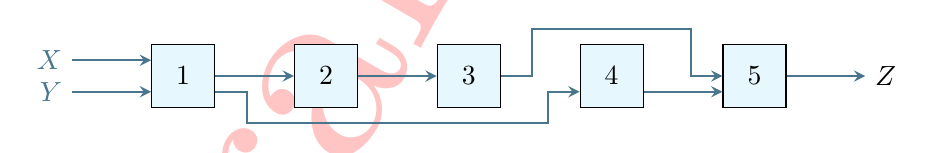
\begin{tikzpicture}[>=Stealth, node distance=1cm,
    startstop/.style = {rectangle, rounded corners, minimum width=3cm, minimum height=1cm, text centered, draw=black, fill=cyan!10},
    process/.style = {rectangle, minimum width=0.8cm, minimum height=0.8cm, text centered, draw=black, fill=cyan!10},
    arrow/.style = {thick,->,>=stealth,darkcyan}]
         % Nodes
        \node (process1) [process] {1};
        \node (process2) [process, right=of process1] {2};
        \node (process3) [process, right=of process2] {3};
        \node (process4) [process, right=of process3, bend left] {4};
        \node (process5) [process, right=of process4, bend right] {5};
        \node (output) [right=of process5] {$Z$};

        % Arrows
        \draw [arrow] ($(process1.west)+(-1,0.2)$) node[left]{$X$} -- ($(process1.west)+(0,0.2)$);
        \draw [arrow] ($(process1.west)+(-1,-0.2)$) node[left]{$Y$} -- ($(process1.west)+(0,-0.2)$);
        \draw [arrow] (process1) -- (process2);
        \draw [arrow] (process2) -- (process3);
        \draw [arrow] (process3) -- ($(process3.east)+(0.4,0)$) -- ($(process3.east)+(0.4,0.6)$) -- ($(process5.west)+(-0.4,0.6)$) -- ($(process5.west)+(-0.4,0)$) -- (process5);
        \draw [arrow] (process5) -- (output);
        \draw [arrow] ($(process1.east)+(0,-0.2)$) -- ($(process1.east)+(0.4,-0.2)$) -- ($(process1.east)+(0.4,-0.6)$) --  ($(process4.west)+(-0.4,-0.6)$) -- ($(process4.west)+(-0.4,-0.2)$) -- ($(process4.west)+(0,-0.2)$); %硬编码!
        \draw [arrow] ($(process4.east)+(0,-0.2)$) -- ($(process5.west)+(0,-0.2)$);

        % Additional connection (optional)
        %\draw [arrow, dashed] (process1) -| (process4);
    \end{tikzpicture}
\end{figure}
}

明确静态流水线的特征是\Emph{加法和乘法运算不能同时进行}。

对于此题,我们可以连续计算 $a_1b_1$、$a_2b_2$、$a_3b_3$、$a_4b_4$ 共 4 次乘法运算(将 4 个乘积分别记为 $c_1,c_2,c_3,c_4$),随后进行 $(a_1b_1 + a_2b_2) + (a_3b_3 + a_4b_4)$ 共 3 次加法运算,相当于总共 7 条指令:

\begin{table}[htb]
    \centering
    \begin{tabular}{ccccc}
        1: & \verb|mul| & $c_1$ & $a_1$ & $b_1$ \\
        2: & \verb|mul| & $c_2$ & $a_2$ & $b_2$ \\
        3: & \verb|mul| & $c_3$ & $a_3$ & $b_3$ \\
        4: & \verb|mul| & $c_4$ & $a_4$ & $b_4$ \\
        5: & \verb!add! & $S_{12}$ & $c_1$ & $c_2$ \\
        6: & \verb!add! & $S_{34}$ & $c_3$ & $c_4$ \\
        7: & \verb!add! & $S$ & $S_{12}$ & $S_{34}$ \\
    \end{tabular}
\end{table}

根据本题题设,可以提炼出如下规则:
\begin{itemize}
    \item 第 4 条指令执行完毕以后,第 5 条指令才能开始\textcolor{gray}{(因为静态流水线)}
    \item 第 1、2 条指令执行完毕以后,第 5 条指令才能开始\textcolor{gray}{(因为需要 $c_1,c_2$ 值,「写后读」相关)}
    \item 第 3、4 条指令执行完毕以后,第 6 条指令才能开始\textcolor{gray}{(因为需要 $c_3,c_4$ 值,「写后读」相关)}
    \item 第 5、6 条指令执行完毕以后,第 7 条指令才能开始\textcolor{gray}{(因为需要 $S_{12},S_{34}$ 值,「写后读」相关)}
\end{itemize}

\backgroundsetup{contents=
\includegraphics{下半示例.png}, center, scale=1, angle=0, opacity=1}
\BgThispage
如此可以做出时空图:
\begin{figure}[htb]
    \centering
    \begin{tikzpicture}[>=Stealth, xscale=0.7, yscale=0.7]
        \draw[brown!50, thin] (0,0) grid (15,5);
        \draw[->] (0,0) -- (17,0) node[above, font=\small] {时间$(\Delta t)$};
        \draw[->] (0,0) -- (0,6) node[left, font=\small] {空间};
        \foreach \i in {1,...,15} {
            \node[below, font=\small] at (\i-0.5, 0) {\i};
        }
        \foreach \i in {1,2,...,5} {
            \node[left, font=\small] at (0, \i-0.5) {\i};
        }
        % 填充指令块(配合导言区定义看)
        \drawrecmul{1}{red!40}{1}; 
        \drawrecmul{2}{orange!40}{2};
        \drawrecmul{3}{yellow!40}{3};
        \drawrecmul{4}{SpringGreen!60}{4};
        \drawrecadd{7}{Emerald!40}{5};
        \drawrecadd{8}{NavyBlue!40}{6};
        \drawrecadd{12}{RoyalPurple!40}{7};
    \end{tikzpicture}
\end{figure}

从上面的「彩虹时空图」可以看出,整个流水线经历了 15 个$\Delta t$。

\begin{itemize}
    \item 实际吞吐率 $TP = \dfrac{\text{指令数}}{\text{流水线用时}} = \dfrac{7}{15\Delta t}$
    \item 加速比 $S_p = \dfrac{\text{非流水线用时}}{\text{流水线用时}} = \dfrac{3\times 4\Delta t+4\times 3\Delta t}{15\Delta t} = 1.6$
    \item 效率 $\eta = \dfrac{\text{有效时空区}}{\text{总时空区}} = \dfrac{3\times 4+4\times 3}{15\times 5} = \dfrac{24}{75} = 32\%$
\end{itemize}

\vspace{1em}

{\color{cyan!80!black}
【结论】$TP=\dfrac{7}{15\Delta t}$,$\eta = 32\%$。

\vspace{0.5em}
【点评】这是一道指令流水线的分析题。其中,本题的「静态流水线」是一个坑点,因为它规定了乘法和加法指令不能同时运行,这一点对时空图的影响比较关键。此外,同学们还需要掌握流水线的几个性能指标,如最大吞吐率、实际吞吐率、加速比、效率等。
}


\end{document} 